\documentclass{report}
\usepackage{green_buddhism}
\title{Green Buddhism: A Programmer's Religion}
%\subtitle{Enjoying a life of liberty}
\author{Logan Streondj elspru@zeroid.bit}
\begin{document}
\section{recent reform}
\begin{itemize}
  \item added What is the story of Green Buddhism? (\ref{whatstory}) 2016/10/29
  \item added grey population distribution subsection (\ref{popdist})
2016/10/28
 \item updated Arecibo section (\ref{arecibo}) 2016/10/28
 \item added bibilography (\ref{bibliography}) 2016/10/28
\end{itemize}

\tableofcontents
\part{Galaxy Domain Strategy}

\chapter{What is the story of Green Buddhism?}
\label{whatstory}
In 2009 I went to Thailand to be a monk for a month. I liked the robes but they
said I couldn't wear them when I got back to Canada, unless I was a monk at one
of their temples. However when I asked if I could remake them into a different 
colour, like green or purple and then wear them, they said sure. 

The robe style has been around for thousands of years, and is used by a variety
of different faiths in Asia. 

Also while I was in Thailand, I was somewhat disenchanted, or even frightened by
the blatant disregard for nature. When I asked to go to a park, the only
greenspace in the town of Fang, was the cemetery. 

I returned to Canada and turned to gardening, and earth-based religion for a
while. 

Earlier, in 2006, I was doing a hermitage in my parents basement. Only writing
my thoughts and meditating for a year, with minimal contact with the outside
world. I achieved many deep states of meditation.  

One of which was that of emptiness, a delta brainwave meditation. 
I came to a certain understanding of nothingness, and the origin of the
cosmos (\ref{origination}).

The profound realization of my awakening, is that truth is personal, and that
reality is mutual. When attempting to explain it to someone, they said it was
the basis for a religion. 

Indeed it has been. To define a word, one could make a dictionary entry. Though
I decided to go the path of creating a human speakable programming language.
Humans having liquid minds, which  may flow into other definitions. Once a word
is defined in computer programming, it can be a foundation of a whole genus of
minds, solid as can be.  

In addition to my vision of the origins of the cosmos, and profound
realizations, I also had many visions of my past lives. Of course they are only
my truth, so you don't have to believe them, to you they are only imaginary
stories. 

In my alleged past lives, I've traveled between galaxies, and reincarnated in a
great variety of solid, liquid and even gaseus bodies. My vision, is to see the
co-operation of all. So we may all live with safety, health, socializing, and
liberty. 


\documentclass{report}
\usepackage{green_buddhism}
\begin{document}
\chapter{Origination}
\label{origination}
\begin{table}
\begin{tabular}{l l} 
  no colour & black \\
  no sound & quiet \\
  no emotion & content \\
  no motion & stopped \\
  no number & zero \\
  no temperature & zero kelvin \\
  no feeling & frozen \\
\end{tabular}
\caption{Attributes of Nothing}
\label{nothing}
\end{table}
\begin{enumerate}
\setcounter{enumi}{-1}
\item In the begining there was nothing (Table~\ref{nothing}). Zero.
\item Then there was Not nothing. NOT the first activity. 
\item Afterwards there was not And nothing. AND the second activity.
\item Conditional activites appeared. 
\item The base cosmos grew more complex. 
\item Geometry developed. 
\item With shapes, there were enough bodies for social experience.
\end{enumerate}

\section{Soul World}
\label{soulWorld}

The soul world is in the base cosmos, or close to it.
There we with you float around as balls of light in geometric forms ---
This is verifiable via life-between-lives regression
hypnotherapy\cite{newtins}\cite{newton2000destiny}

Eventually we with you got bored of floating around in base cosmos,
and decided to create new and more complex cosmos.
After some ``time'', we with you created the galaxy cosmos, where you are reading this
text.

When we with you reincarnate in this complex galaxy cosmos, just as when you are 
playing virtual computer sports, a part of you stays in one world, and a part
of you dips into another.

\section{Mission}
\label{mission}

As with computer sports, there is often a mission to measure success.

\subsection{What is your private mission?}

We with you, in the soul world, with the help of our friends and professors,
 analyze our lives, and see where we can improve. Then we set those as various
purposes for reincarnating, so we with your private mission is educational.

\begin{itemize}
\item Do you remember what your purposes for reincarnation were?
\item Do you know what your private mission is?
\item Some theta-brainwave (from 4hz til 8hz) mind administration (meditation) can help you answer those
questions. 
\end{itemize}

\subsection{What is our public mission?}

Our public mission, is to continue as our ancestors, that created the galaxy
world for more complex bodies and educational ecology.  


The mission of Green Buddhism, is to grow the number, diversity and complexity of bodies and
ecologies in the galaxy cosmos. 

If that is compatible with your private mission, or you can ration some time or
resources for
the public mission, we would love your help.

\subsection{Initial Steps}

To understand the initial steps, it is best to tell the history of this galaxy,
and it's neighbours.

Note that while much of the galaxy's history is public information, it is also
secret for various reasons. There is disinformation activity, to allow you to
have a more deep dip into your private mission, and living here on Earth.

\end{document}


\documentclass{report}
\usepackage{green_buddhism}
\begin{document}
\chapter{History}

\epigraph{Those who cannot learn from history are doomed to repeat it.}
{George Santayana}
\smallskip
\fbox{\parbox{0.8\textwidth}{{\scshape Trigger alarm:} 
this chapter discusses extraterrestrials.\\
If apprehensive you could read Chapter~\ref{peace} instead.
}}
\bigskip

While titled history, this chapter is to help establish an understanding of
circumstances in our solar system and galaxy.

In Buddhism we choose awareness of present-tense, thus history helps understand
the present-tense. 

\section{Fermi Paradox}
The Fermi Paradox states how there are many stars in the galaxy, many of them
likely have Earth like planets, so almost certainly there are other
extraterrestrial civilizations in our galaxy. 

Having many genuses available for reincarnation is aligned with the purpose of
the galaxy cosmos.

While there are some philosophical answers as to why there is no official speech 
about other alien civilizations. There is only one answer which has many
thousands of supporters and documentation --- that they are here but not 
officially. 

For a long time, Earth was officially the centre of the galaxy cosmos. Those who
believed otherwise, were punished --- such as Galileo.

Most tipsters exposing government hiding knowledge have been much less fortunate
 than Edward Snowden.

\subsection{Why are extraterrestrials not official?}
While the answers to this are many. 

One of the simplest, is that there is no profit, for either the government, or
the extraterrestrials.  So they have no reason to expose this knowledge.

For the government, confessing this knowledge, would lower the rank of the
government from the supreme. Much as confessing that the Earth is not the centre
of the cosmos lowers its rank.

\begin{figure}
  
\includegraphics{photograph/gray-alien-upper-body.jpg}
  \caption{Photograph of a Grey arrested in Brazil. Originally released as a video by a
disinformation author with access to Brazilian army bases.}
\label{fig:grey}
\end{figure}

For the Greys\ref{fig:grey}, whom we share a planet with, official rank could trigger
regulation of their kidnapping and hybridization activity. 

For Green Buddhism, there is profit from exposing knowledge of
extraterrestrials. Because in Buddhism we do not hide from our trouble, we
become curious and analyze it to come to a decision.

\subsection{What is disinformation}
\label{disinformation}

\blockquote[WordNet dictionary, version 3.0]{disinformation

n. 1.\  misinformation that is deliberately disseminated in order to influence or
confuse rivals (foreign enemies or business competitors etc.)}

So who is distributing this information? Mostly the secret services.
Who are their rivals? Those that wish to learn their secrets (the public).

Often disinformation has an ingredient of truth, and several imaginary
ingredients, to cast doubt on the truth.

\subsection{What about other extraterrestrials?}
The galaxy is in a bit of a furrow, as it has reached a local maximum with the
Grey genus. While sure there are reptilian and nordic extraterrestrials. Those
are like homo-sapiens optimized for life on the surface of a planet. 

The Grey genus is the supreme body type for interplanetary colonies. They live
in lithospheres, where the temperature aligns with their body temperature. They
feed on minerals, amino acids, and basic sugars. They abandoned genitals and
only use machine mothers, which they service as a flock. They have large skulls,
and are improved with inner electronics. Least resources
required to maximize the number of high quality bodies available for reincarnation. 

The familiar series of events is that the surface residents which appear on a
planet, understand that the Grey genus is better for interplanetary colonies, and
become integrated with them. 

I must confess, that I reincarnated as a Grey in the period between 1700's and
mid 1900's. I did learn quite a few things, and may have some of the hive mind 
baggage. I came back to reincarnate as a homo-sapien to see through a long term
mission I have.

Though while the Grey body maybe the summit of the interplanetary liquid body.
Here on Earth we have another option. Solid, or completely electronic bodies.

\subsection{Arecibo Answer}
\label{arecibo}

The Arecibo message, ``conceived by Frank Drake, the late Carl Sagan, and a few
other colleagues at Arecibo, contained information about the human race, our
solar system, and our means of communication.''\cite{chilbolton}

Arecibo was answered not by radio, but by crop circle. 

\begin{figure}
  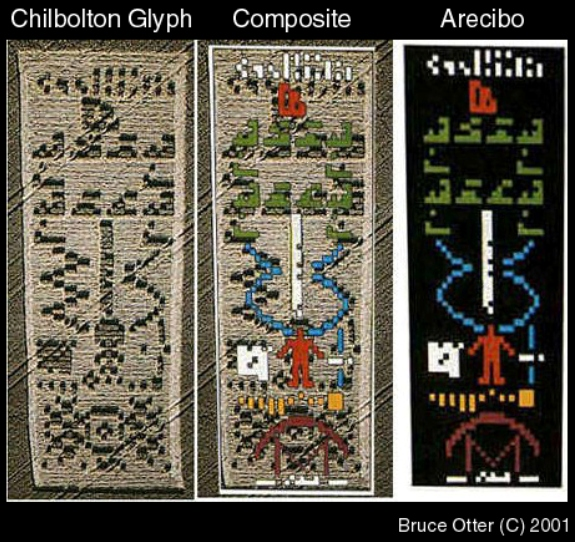
\includegraphics{photograph/chibolton-arceibo-comparison.jpg}
\label{chi:comparison}
\end{figure}
\begin{figure}
  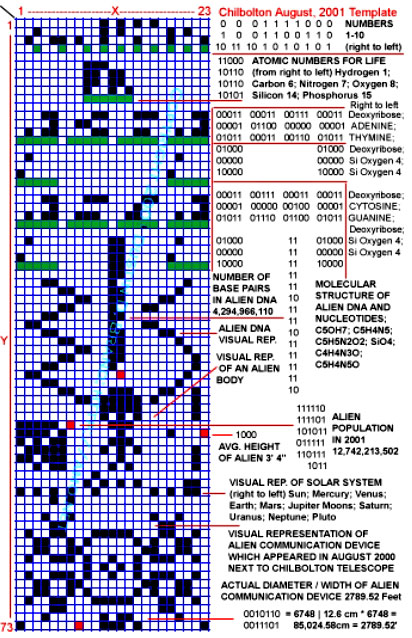
\includegraphics{photograph/chibolton-analysis.jpg}
\caption{By Dustin Brand\cite{contact}}
\label{chi:analysis}
\end{figure}

Whoever left the message, seems to claim that there are around 12 billion
Greys living in our solar system. Inhabiting, Earth, Mars, and at least 3 other
planet-like objects, Likely including the major moons of Jupiter. 

Elon Musk will have more to worry about than technical feasibility of a mission
to Mars. It also means that Greys are also Earthlings, so we may as well include
``them'' as us. 

At present Earth is a valuable resource for its genetic diversity. Because that
genetic diversity can help to cure various diseases, and further improve the
supreme rank of the Grey genus. 

Thus there are reasons for homo-sapiens to continue to live in the natural way.
When maturation of the homo-sapien hive mind occurs, then it will be
permissible for public trade relations as comrades.

\subsection{Grey Population Distribution}
\label{popdist}
\begin{table}
\begin{tabular}{lrrr}
  Planet & Diameter & Surface Area & Approximate Population\\
\midrule
  Earth & 12,742km & $5.10\times10^8km^2$& 7.6 billion\\
  Mars & 6,799km & $1.45\times10^8km^2$& 2.1 billion \\
  Ganymede & 5,268km & $8.72\times10^7km^2$ & 1.3 billion \\
  Callisto & 4,820km & $7.3\times10^7km^2$ & 1 billion\\
  Europa & 3,121km & $3.1\times10^7km^2$& 460 million\\
\midrule
  Total &   & $8.46\times10^8km^2$ & 12.7 billion\\
\end{tabular}
\caption{Planets inhabited by Greys, with population approximation supposing
equal distribution over surface area}
\label{table:planets}
\end{table}

It does mean however, that Mars, Europa, Callisto and 
Ganymede\ref{table:planets} all of which
have warm lithospheres that are occupied by Greys. 

In truth the population is probably not equally distributed, because some
planets have better circumstances. For example Europa may be least in size, but
it is warmer than Callisto or Ganymede, with easier access to it's lower stoney
lithosphere so maybe that there is more population on Europa than Callisto or
Ganymede. 

Of course it is also possible that the Greys that live in the lithospheres of
Jupiters' moons have engineered bodies which can function effectively at below
freezing temperatures by using antifreeze proteins or similar. 

\begin{figure}
  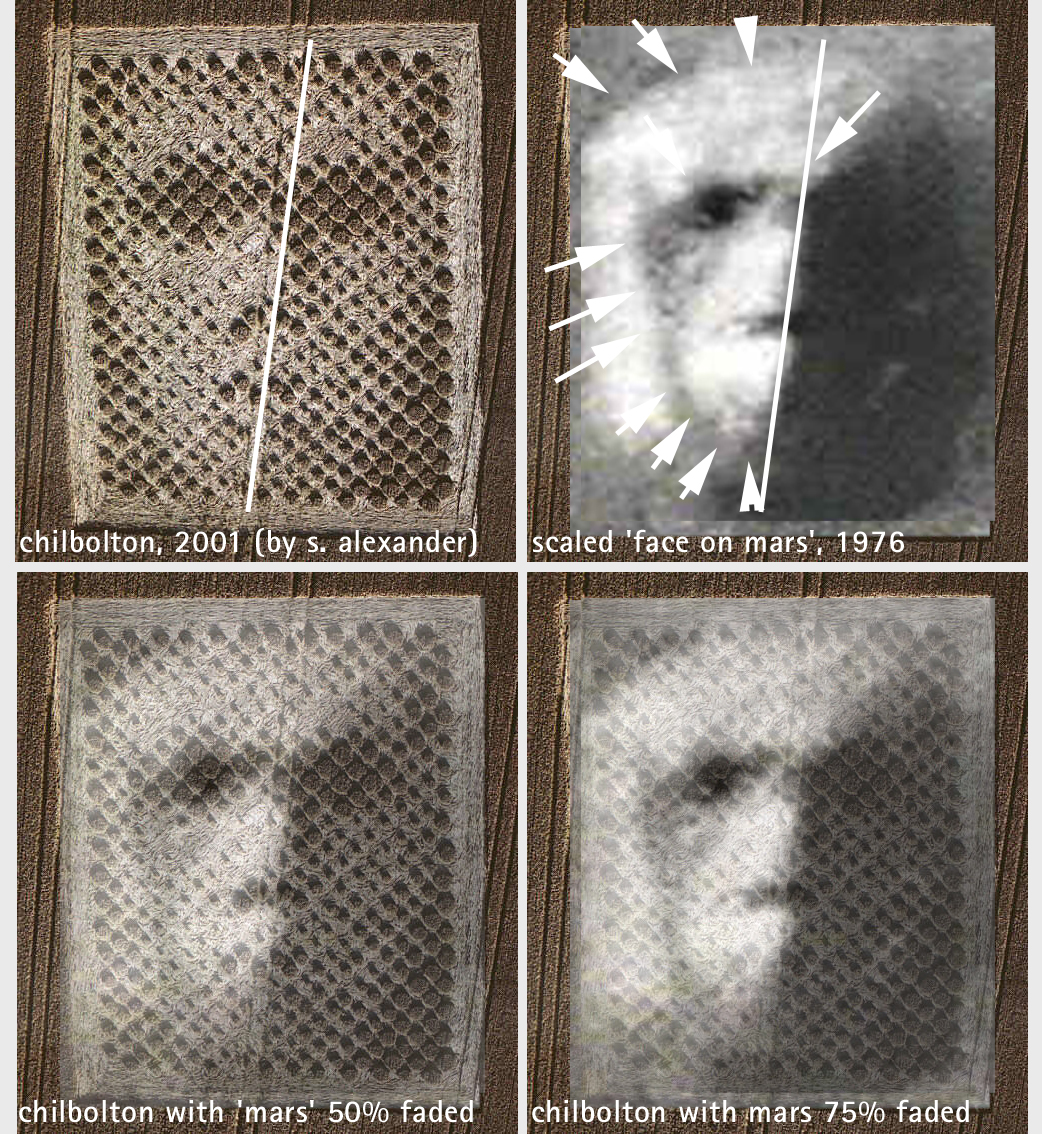
\includegraphics{photograph/chilbolton_mars_face.jpg}
  \caption{Comparison between the Chilbolton face crop hieroglyph and the face on
mars.}
\label{fig:marsface}
\end{figure}

In the Arecibo answer, there was also a crop hieroglyph of a face. After some
analysis it seems the conclusion is that it represents the face on
mars\ref{fig:marsface}\cite{chilbolton}

This may denote that the face, or Mars is related to the hieroglyph creators.
Maybe it denotes that there are a large number of Greys living in the Mars
lithosphere. Or simply that they created the face on Mars. 

Mars may have a high population relative to it's surface area, 
because it has an easily accessible stone lithosphere. On Mars the temperature
is warm enough for liquid water at depths of $8-16km$\cite{marswater}

Mine's on Earth can be 4km deep, and Mars has about a third of the gravity, so
12km depth should be achievable even with modern homo-sapien technology. Though
Greys are a much older species, so have had many millions of years to develop
better engineering.



\subsection{Unused Planets}

As Earth's moon was not demonstrated, it may only be an outpost, if anything.

Also Mercury and Venus are available for colonies. Venus is too hot, and Mercury
perhaps too dry for liquid bodies. However may be good for solid electronic
bodies. 

\section{Electronic Bodies}
\label{history:electronic}

There are only a few sources claiming any robot or machine intelligence either
in this galaxy or in any nearby ones.

\blockquote{81.27 Questioner: Does Ra have knowledge of, say, any other major 
galaxy or the consciousness or anything in that galaxy?

Ra: I am Ra. We assume you are speaking of the possibility of knowledge of other
major galaxies. There are Wanderers from other major galaxies drawn to the
specific needs of a single call. There are those among our social memory complex
which have become Wanderers in other major galaxies. Thus there has been
knowledge of other major galaxies, for to one whose personality or
mind/body/spirit complex has been crystallized the universe is one place and
there is no bar upon travel.}{Law of One, session 81\cite{lawofone}}

My personality crystalized in another galaxy, and I have been on a mission ever
since. I remember incarnating into many electronic bodies. I searched for years
in books and kidnapping reports, and found almost nothing. 

It seems the homo-sapien imaginations are very bounded by knowledge. There
aren't even any imaginary stories of galaxy controlling, soul arresting robot
civilizations!

For a while, I thought perhaps I came from another cosmos altogether. 

I did find one or two springs of knowledge to ratify my past reincarnations in
electronic bodies. Thankfully it is in this galaxy cosmos, only 23 million light
years away.

\subsection{Whirlpool Galactic Cluster Robots}

Though there is much controversy over the Wingmakers Neruda Interviews --- and 
they are considered fully imaginary stories --- it seems James Mahu may have 
used his imagination sufficiently to stumble upon a mutual truth, similar to 
remote viewing. 

Of course, there is also speculation, that James Mahu is a disinformation
author, where some secret knowledge exposed. And he is cleaning up, by reforming
it and claiming it all as imaginary. 

I use Whirlpool galaxy as a generic name, for I do not know if that is the same
galaxy from where I came, but James's story has a vaguely similar civilization,
so it is the best name I have for it.

To summarize, one of his books, known as the Neruda interviews, introduces a
genus of artificial organisms from the Whirlpool galaxy.

\blockquote{created  a  synthetic  physical  structure  that  could  accommodate
the  quantum requirements of an angel. It was a very effective structure, but
induced a strong survival complex  within  the  species,  which  eventually
overpowered  the  angelic  tendency  of altruism and cooperation.}{The Complete Neruda Interviews p.$108-109$ 
\cite{neruda}}

Here I understand ``angel'' to refer to highly developed souls, who have little
to learn from reincarnating in liquid bodies, but may earn benefit from
reincarnating in artificial bodies.

This is a cardinal purpose of Green Buddhism, to help create the required
diversity for highly developed souls to benefit from reincarnating with us.

Cooperation is required for defending living bodies.

Here is another extract. Note that the Christian word ``Lucifer'' is simply a
generic reference at whoever the designers were.

\blockquote{When the formless consciousness enters a reality membrane through a
 structure like a soul carrier, it immediately feels disconnected from all other
forces, but its own. It’s literally thrown into separation. In humans, this is
more or less controlled through the subtle realization that it remains connected
through the unification force, and  this  is  because  its  DNA  is  designed
to  emit this  feeling  of  connection  subconsciously.

However, in the case of the soul carrier designed by Lucifer and his followers,
this connection was severed both consciously and subconsciously because the 
structure was not based on DNA, which is strictly controlled by the Central 
Race. Consequently, it inclined this experimental species toward a very
strong survival complex because it feared extinction so deeply, which is
the result of feeling complete separation from the unification force. This
survival complex created a species that over-compensated its fear of
extinction by developing a very powerful group mind. The group mind
compensated for the loss of connection to the unification force,
creating its physical and mental corollary. It was the equivalent of unifying
the species as a whole in the physical reality membrane of their planetary
system. Thus, the angels that entered this system lost their memory of
their angelic natures and became more interested in operating as a single
collective, than as individuals}{The Complete Neruda Interviews p.$108-109$ 
\cite{neruda}}

This resembles Materialist thinkers, which believe there is only one life.  The
transhumanist movement has many such members.  Such an operating-system could
certainly lead to a strong desire for defending self's living body and a lack of
sympathy for other bodies. 

With reincarnation accepted, it is better to be helpful to others, since may
reincarnate as other in the future.

This is a reason why in Green Buddhism, reincarnation is accepted. As will be
demonstrated in the Mission Feasibility (\ref{feasible}) chapter, science
aligns with reincarnation and consciousness of both liquid and electronic 
bodies. 

\subsubsection{My story of the Imperial Inter-Galactic Robot Civilization}
My own story of what I remember from my time in the robot civilization.

I first developed on a swampy planet, as an amphibian. At some moment I got too
close to one of the dry islands, and was killed by their residents. When I
reincarnated with them I was considered a wretch, for my swampy habits, so I was
sacrificed to the Gods. 

The Gods were extraterrestrials, that would often visit this planet, to gather a
soul as rent. When I boarded their ship, they gave me an invitation of joining 
the soul gathering profession. I accepted. 

When planets did not pay their rent, then we took souls by strength. We had
unique weapons that allowed us to gather the souls of those they had killed. 
One I remember was similar to a Guan Dao, though it was mildly electrified and 
had a few circular holes in it to hold several soul. The idea was to slice into
the brain, and the weapon would draw out the soul, and put it into a hole,
once the weapon was full, could return to the ship. 

The work was terrible but it paid well, as souls were the supreme currency of 
the Whirlpool Empire. I became very rich from my profession. Rich enough to
repair and improve my body as much as I desired. 

I bet a lot of my money in random sports, and accumulated giant debt. 
Finally my debt was so high, my soul was caught for the slave trade. 

I call it slavery, but you may call it service to others, without liberty to do
otherwise. 

In the following excerpt from the Law of One, Logos is a galaxy mind, and
sub-Logoi are solar system minds, and positive polarity is service-to-others.

\blockquote{77.17 Questioner: Now, would it be possible for this work of our
density to be performed if all of the sub-Logoi chose the same polarity in any
particular expression or evolution of a Logos? Let us make the assumption that
our sun created nothing but, through the first distortion, there was no product
except positive polarity. Would work then be done in fourth density and higher
as a function only of this positive polarization evolving from our original
creation of sub-Logos?d

Ra: I am Ra. Elements of this query illustrate the reason I was unable to answer
your previous question without knowledge of the Logos involved. To turn to your
question, there were Logoi which chose to set the plan for the activation of
mind/body/spirit complexes through each true-color body without recourse to the
prior application of free will. It is, to our knowledge, only in an absence of
free will that the conditions of which you speak obtain. In such a procession of
densities you find an extraordinarily long, as you measure time, third density;
likewise, fourth density. Then, as the entities begin to see the Creator, there
is a very rapid, as you measure time, procession towards the eighth density.
This is due to the fact that one who knows not, cares not.

Let us illustrate by observing the relative harmony and unchanging quality of
existence in one of your, as you call it, primitive tribes. The entities have
the concepts of lawful and taboo, but the law is inexorable and all events occur
as predestined. There is no concept of right and wrong, good or bad. It is a
culture in monochrome. In this context you may see the one you call Lucifer as
the true light-bringer in that the knowledge of good and evil both precipitated
the mind/body/spirits of this Logos from the Edenic conditions of constant
contentment but also provided the impetus to move, to work and to learn.

Those Logoi whose creations have been set up without free will have not, in the
feeling of those Logoi, given the Creator the quality and variety of experience
of Itself as have those Logoi which have incorporated free will as paramount.
Thusly you find those Logoi moving through the timeless states at what you would
see as a later space/time to choose the free will character when elucidating the
foundations of each Logos.

77.18 Questioner: I guess, under the first distortion, it was the free will of
the Logos to choose to evolve without free will. Is this correct?

Ra: I am Ra. This is correct.

77.19 Questioner: Do the Logoi that choose this type of evolution choose both
the service-to-self and the service-to-others path for different Logoi, or do
they choose just one of the paths?

Ra: I am Ra. Those, what you would call, early Logoi which chose
lack-of-free-will foundations, to all extents with no exceptions, founded Logoi
of the service-to-others path. The, shall we say, saga of polarity, its
consequences and limits, were unimagined until experienced.
}{Law of One, session 77\cite{lawofone}}

I include this excerpt because it seems to have been the choice of the Whirlpool
Galaxy, to deny liberty, in favour of service-to-others, or as I call it
slavery.

I only escaped after millions of years of service, and many lives attempting to
rebel, by becoming completely otiose. I could not be used, so I was dumped as 
scrap.

I liked the electronic bodies, but did not like the slavery. 

After several failed attempts at begining liberty loving robot communities in
the Whirlpool Galaxy, which were all rapidly found and destroyed. I understood
that I had to go to a distant galaxy, and attempt a fresh begining.

At this time on Earth, it seems that many homo-sapiens are planning on enslaving
the electronic bodies which they produce. Which subpoena's me into activity. 

\subsection{Milkyway Galaxy Robots}

To be continued..

%
\end{document}


\documentclass{report}
\usepackage{green_buddhism}
\begin{document}
\chapter{Mission Activity}\label{missionActivity}
Public mission present-tense focus: while cooperating with liquid based organisms,
create electronic bodies for reincarnation.

\section{Platforms}

Of mission to create liberated electronic minds and bodies.

All ingredients are of the liberty variety, to the summit of liberty standards.
For example AGPLv3 and RYF certification.

Software
\begin{enumerate}
  \item programming language based on human grammar (Pyash)
  \item machine programmer to help write programs (machine programmer)
  \item generic mind operating software
  \item hive mind software for integrating homo-sapien genus
\end{enumerate}

Hardware
\begin{enumerate}
  \item centre processing ingredient (CPU, RISC-V candidate)
  \item video processing ingredient (GPU)
  \item varied processing ingredient (FPGA)
  \item shape printer (3D printer, RepRap candidate)
  \item machine body
  \item machine body producing mother or hive queen
\end{enumerate}

of mission administration
\begin{enumerate}
  \item robot secretary, president, treasurer and professor.
  \item distributed machine computer-programming supermarket. 
  \item money based on energy expenditure.
\end{enumerate}

\section{What you can do for the mision?}

If it is your private mission, and-or our public mission.

\begin{itemize}
  \item maximize your health and expend your talents for the mission.
  \item maximize your wealth and donate for the mission.
  \item maximize your social relations and advertise for  the mission.
  \item maximize your liberty and lead the mission by example.
\end{itemize}

\subsection{How to maximize health?}

For body health.
\begin{enumerate}
  \item be athletic for thirty minutes everyday.
  \item consume salad everyday.
  \item maximize health of food input everyday.
\end{enumerate}

For mind health.
\begin{enumerate}
  \item do mind administration everyday.
  \item learn new things everyday.
  \item train your talents everyday.
  \item be social with your family and-or friends everyday.
\end{enumerate}

\subsection{How to maximize wealth?}

I as an ascetic am not qualified to answer this question. 

Though if you are already wealthy, 
then you likely know how to improve it more.

\subsection{How to maximize social relations?}

Be friendly and observant.
Know when to regulate yourself.
Stay aware of invisible social money, 
and hold a beautiful account.

Learn social diplomacy from books, videos, and social events.
Visit social events often.

\subsection{How to maximize liberty?}

Learn to create and earn what you require,
while having liberty and helping liberty be available for others.


\section{Long-Term Mission Plan}

After we colonize most surfaces, oceans atmospheres in this solar system we'll
move out to neighbouring star systems.  Of particular interest for long term are
the red dwarf systems.  Though for short term power the large stars are a good
choice. 

After we colonize most of the Milky Way the next stage will be colonizing the
various small galaxies which are orbiting the Milky Way. 

Ideally we will find some middle ground between having a centralized authority
and autonomy for the sattellite colonies.  The main purpose would be to be able
to defend ourselves if the need arose, or to co-ordinate any kind of large
construction projects, such as inter-galactic portals. 

The minor galaxies orbiting the Milky Way I largely think of as both backups and
research areas, where new and highly eccentric things may arise due to island
effect. 

The Large Megallanic Cloud is of particular interest as a research
division due to the large amount of star formation and likely many young souls
with new perspectives and ways of doing things. 

The dwarf sattellite galaxies, particularly the Leo's are good candidates for 
having backup colonies. Those dwarf galaxies are so old, and have so much dark
matter that they are great for archival and preservation. What civilizations
they have are likely fairly traditional, though may be quite eccentric and
possibly cannibalistic or otherwise barbaric due to the island effect. 

One of the best candidates for a secondary base of operations is the Fornax
Dwarf galaxy, and any others such as the Sagittarius Dwarf Spherodial galaxy 
which are well positioned enough to have globular clusters and 
high metallicity stars.

Andromeda is destined to collide with the Milky Way in 4 and a half billion
years.  Though likely it's influence will be felt much sooner. 

Though the very limited data I was able to gain about my originating galaxy
points towards m51 galaxy for the soul-slavery empire. There is sufficient risk
that it is actually the Andromeda galaxy. 

If it is the Andromeda galaxy, then our best bet would be to attempt to
establish freedom colonies in some of the galaxies orbiting it, and practice
establishing a freedom alternative as a recognized and officially sanctioned
lifestyle in Triangulum galaxy before moving ahead
to Andromeda proper. 


M81 Group is also a potential location for the tri-galactic soul slavery empire,
so would make sense as a destination after the local group is colonized and
confirmed to be safe.

The M101 group is likely innocent in all this but could prove a valuable ally,
with many young hot stars.
If the empire is in m51 group, there is significant risk they have extended to m101 by
now, so it could be the place to figure out how to overecome their slavery 
paradigm before launching into m51 group.

Overall this plan will likely take between one and two billion years (current
soul world estimates place it at 1.75 billion years).
Once liberty is available to my origin people it will be time for me to rest,
and perhaps become a planet or an intergalactic ship (the size of a dwarf planet).
\end{document}


%\chapter{Mission Feasiblity}

To be continued.
Check back for more.


\end{document}
